\subsection{Structure of the consumer client}\label{ssec:consumer_client_structure}
The consumer client is a proof of concept of implementing the use of the REST API.
The consumer client also helped in the process of discovering errors and missing functionalities.
It is build to showcase the different functionalities and the different types of data the REST API can produce.

\subimport{../}{consumer_client_fig.tex}

In \cref{fig:consumer_client} the overall layout of the consumer client can be seen.
When a user first enters the consumer client, a login screen will be presented as can be seen in \cref{fig:ConsumerClientLogin}.
\begin{figure}[h]
    \centering
    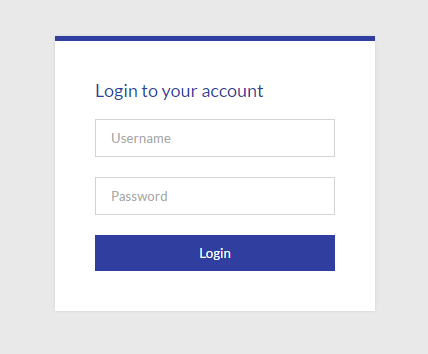
\includegraphics[width=0.75\textwidth]{img/ConsumerClientLogin.png}
    \caption{The login page for the consumer client.}
    \label{fig:ConsumerClientLogin}
\end{figure}

\bigskip
When a user is logged in he/she is firstly presented for an overview of the dashboard.

\begin{figure}[h]
    \centering
    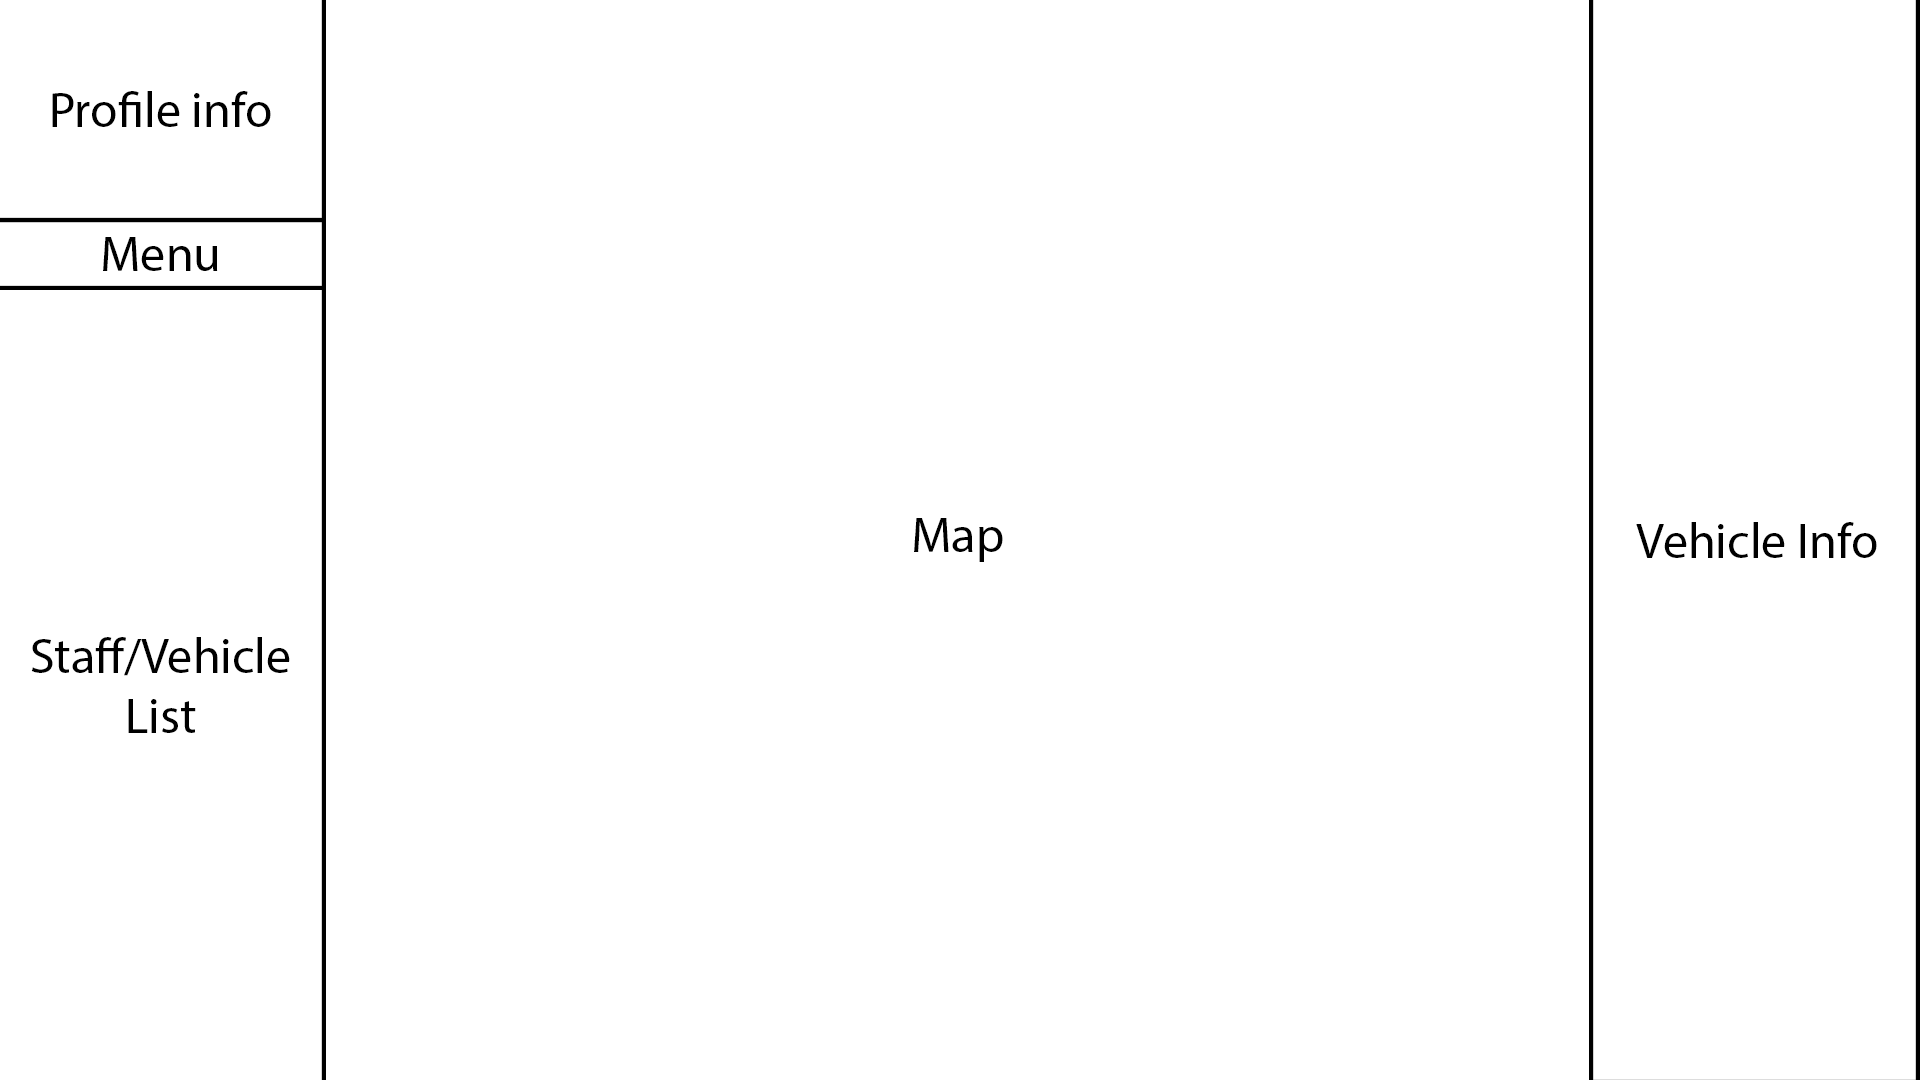
\includegraphics[width=0.75\textwidth]{img/ConsumerClientWText.png}
    \caption{A structural overview of the dashboard for the consumer client.}
    \label{fig:ConsumerClientLayout}
\end{figure}

As can be seen in \cref{fig:ConsumerClientLayout}, the user can see his/her user information in the top left corner, this information is fetched through the REST API.
More precisely the users name, username and status is fetched.
\begin{figure}[h]
    \centering
    
\includegraphics[width=0.75\textwidth]{img/ConsumerClientProfile.png}
    \caption{A display of how the profile information area looks.}
    \label{fig:ConsumerClientProfile}
\end{figure}
In the example, which can be seen in \cref{fig:ConsumerClientProfile}, the users status can be wither a user or a super user.
The user's image is also fetched through the REST API, the image is Base64 encoded and represented as a background image, however if the user has no image, a default image will be shown.

\bigskip
Beneath the profile information a small menu can be seen, \cref{fig:ConsumerClientLayout}, this menu is used to navigate between two lists.
A list containing all the employees of the designated company, and another list which represents all the vehicles which is connected to the company.

\begin{figure}[h]
    \centering
    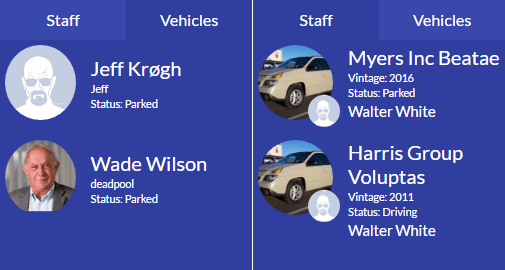
\includegraphics[width=0.75\textwidth]{img/displayOfMenuesInConsumerClient.png}
    \caption{Display of what the different employee and vehicles can contain.}
    \label{fig:ConsumerClientMenus}
\end{figure}

In the list of all the employees, the name, username, image and the current status of the driver can be seen.
This status is not like the status shown in the profile information, this status is whether the users are currently driving or parked.
If a user is currently driving, an image of the vehicle will be shown next to the user's image.
The list of users is automatically to fit to the newest data from the REST API.

Likewise in the employee/vehicle list, some information can be seen of each vehicle.
This information consists of the make and model, an image of the vehicle and whether the vehicle is currently driving or parked.
If the vehicle is currently driving, a small image of the driver will be shown next to the image of the vehicle.

If the user of the dashboard clicks on either a vehicle or a driver, which is currently driving, the map will automatically center the map around the currently active route the vehicle is driving.

\bigskip
The dashboard also contains an interactive map, the user is able to zoom and move the map, and through the REST API, the consumer client is able to show the currently active vehicles within the currently visible part of the map.
All the routes which are shown will continually be updated, and movement can be shown in real--time.
All vehicles on the map will by default be represented by a small yellow truck, however if the vehicle has a custom image, the image will be loaded and shown instead of the yellow truck\footnote{\url{https://www.iconfinder.com/icons/22999/lorry_transport_transportation_truck_vehicle_yellow_icon}}.

\begin{figure}[h]
    \centering
    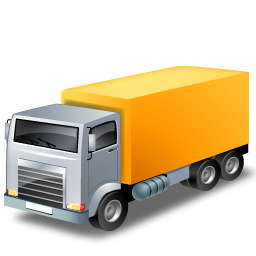
\includegraphics[width=0.75\textwidth]{img/Truck_Yellow.png}
    \caption{The default yellow truck which will be seen on the map, if the vehicle has no custom image.}
    \label{fig:ConsumerClientYellowTruck}
\end{figure}

All the routes which are drawn on the map are polypaths which are drawn between the different GPS coordinates which the vehicle itself sends to the REST API.
A polypath is a line drawn on the interactive map, between an ordered list of GPS coordinates.


\bigskip
\begin{figure}[h]
    \centering
    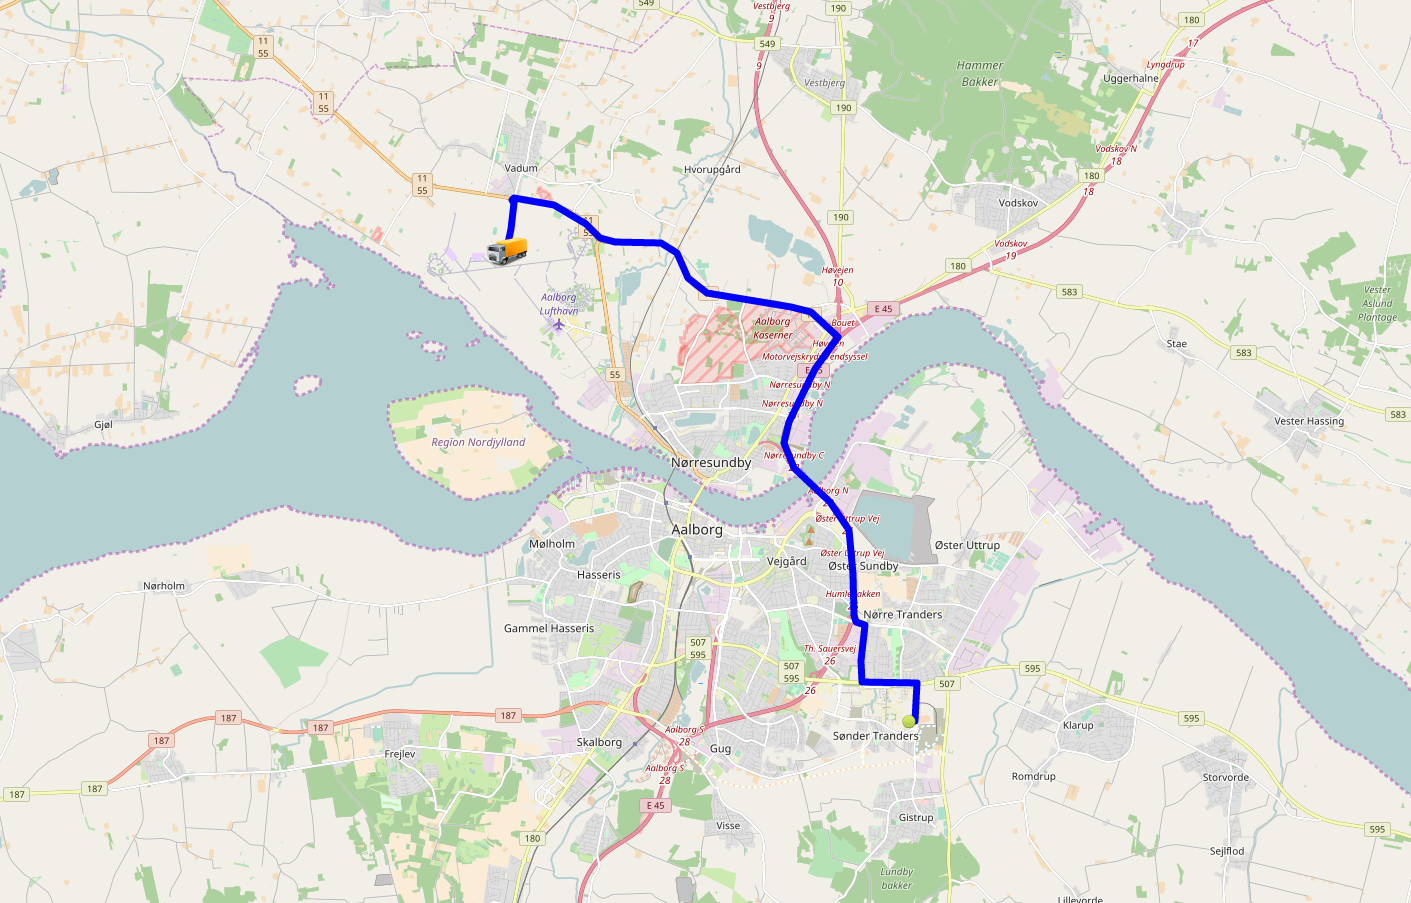
\includegraphics[width=0.75\textwidth]{img/ConsumerClientMap.png}
    \caption{An example of how the interactive map could look. Displaying a theoretical route.}
    \label{fig:ConsumerClientMap}
\end{figure}
When a vehicle is clicked, a menu in the right side will be shown, this menu currently contains nothing, but could be used to show more advanced vehicle information, for instance live vehicle data, and previous routes the vehicle has driven.

\bigskip
The consumer client allows for a fast overview of the entire fleet, while also granting the company an opportunity to track its vehicles in real--time on the map and show the current information at the same time.

Since the company is able to track the vehicles in real--time, the consumer client could be used to help prevent future damages to the vehicles.
This can be done by analysing either the real--time data, or by looking for anomalies or deviations in the data from previous routes.

\fxnote{vise noget kode i løbet af afsnittet?}
